\documentclass[10pt]{beamer}
\usepackage[utf8]{inputenc}
\usepackage[T1]{fontenc}
\usepackage[francais]{babel}
\usepackage{graphicx}
\usetheme{Luebeck}

\usepackage{tikz}
\usetikzlibrary{arrows}
\usetikzlibrary{positioning}
\usetikzlibrary{decorations.markings}
\tikzstyle{nodeStyle}=[rectangle,rounded corners, text width=2cm, text centered]

\title{Introduction à la Recherche en Laboratoire }
\subtitle{Solutions de viscosité et schémas numériques associés}
\author{Gaétan Bahl \\ Encadrant : Emmanuel Maître}\institute{Grenoble INP Ensimag \\ Laboratoire Jean Kuntzmann -- Équipe EDP}

\AtBeginSection[]
{
    \begin{frame}
    \frametitle{Sommaire}
    \tableofcontents[currentsection]
        \end{frame} 
}

\AtBeginSubsection[]
{
    \begin{frame}
    \frametitle{Sommaire}
    \tableofcontents[currentsection, currentsubsection ]
        \end{frame} 
}


\begin{document}


\begin{frame}
\titlepage
\end{frame}

\section{Introduction}
\begin{frame}
\frametitle{Sujet de l'IRL}

\begin{itemize}
\item Comprendre la notion de solution de viscosité d'équation aux dérivées partielles

\item Trouver dans la littérature un problème à résoudre numériquement

\item Implémenter la résolution dans un langage de programmation au choix 
\end{itemize}

\end{frame}

\section{Solutions de viscosité}

\subsection{Rappels}
\begin{frame}

\frametitle{Équations aux Dérivées Partielles}

\begin{block}{Équation aux Dérivées Partielles}
Une équation aux dérivées partielles d'ordre $k$ est une équation liant une fonction
et ses dérivées jusqu'à l'ordre $k$. Par exemple :

$$k=2, \;  F(x,u,Du,D^2u) = 0, x\in \Omega \subset \mathbb{R}^n $$

où $F : \Omega \times \mathbb{R} \times \mathbb{R}^n \times \mathcal{M}_{n,n} \to \mathbb{R}$.
\end{block}

\begin{block}{Exemple d'EDP : Équation de la chaleur}
$$\frac{\partial u}{\partial t} - \Delta u = 0$$
\end{block}

\end{frame}

\begin{frame}
\frametitle{Solution classique}
\begin{block}{Solution classique d'une EDP}
Une fonction $u : \Omega \to \mathbb{R}^n$ est appelée \emph{solution classique} d'une EDP d'ordre $k$ si elle est $\mathcal{C}^k$ et satisfait l'EDP $\forall x \in \Omega$.
\end{block}

\begin{block}{Problème des solutions classiques : Équation Eikonale}

Toutes les EDP n'admettent pas nécessairement une solution classique, par exemple :

$$ |Du| = 1 $$

\end{block}

\end{frame}

\subsection{Définition}

\begin{frame}
\frametitle{Sous-Différentielle}
\begin{block}{Sous-gradient}
Un vecteur $p$ est un sous-gradient de $u$ en un point $x$ si la droite orientée par $p$ est tangente sous la courbe de $u$ en $x$.
On note l'ensemble des sous-gradients de $u$ en $x$ : $D^{-}u(x)$.
\end{block}
\begin{figure}
\begin{center}
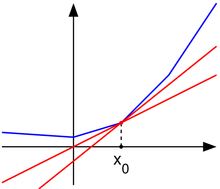
\includegraphics[scale=0.4]{sousdiff.png}
\caption{Exemple de sous-gradients}
\end{center}
\end{figure}
\end{frame}

\begin{frame}

\frametitle{Solution de viscosité}
\begin{block}{Sous-solution de viscosité}
Une fonction $u$ est une \emph{sous-solution de viscosité} d'une EDP si 
$$F(x,u(x),p) \leq 0, \forall x \in \Omega, p \in D^{+}u(x) $$
\end{block}

\begin{block}{Sur-solution de viscosité}
Une fonction $u$ est une \emph{sur-solution de viscosité} d'une EDP si 
$$F(x,u(x),p) \geq 0, \forall x \in \Omega, p \in D^{-}u(x) $$
\end{block}

\begin{block}{Solution de viscosité}
Une fonction $u$ est une \emph{solution de viscosité} si elle est à la fois
une \emph{sur-solution} et une \emph{sous-solution}.
\end{block}
\end{frame}

\subsection{Exemple}

\begin{frame}
\frametitle{Exemple en 1D}
\begin{block}{Équation eikonale}
$$|Du| = 1 $$
\end{block}

\begin{figure}
\begin{center}
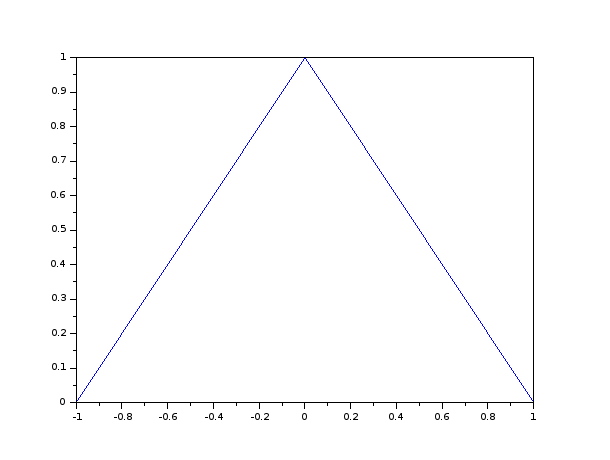
\includegraphics[scale=0.22]{eikonale.png}
\caption{Solution de viscosité de l'équation eikonale}
\end{center}
\end{figure}

\end{frame}

\section{Équation de Monge-Ampère et transport optimal}

\subsection{Présentation du problème}

\begin{frame}
\frametitle{Problème choisi}

Problème de transport optimal en 2D \\

    Déplacement d'une mesure de probabilité \\

    D'après un article de Benamou, Froese, Oberman.

    \bigskip

    \begin{figure}
    \begin{center}
    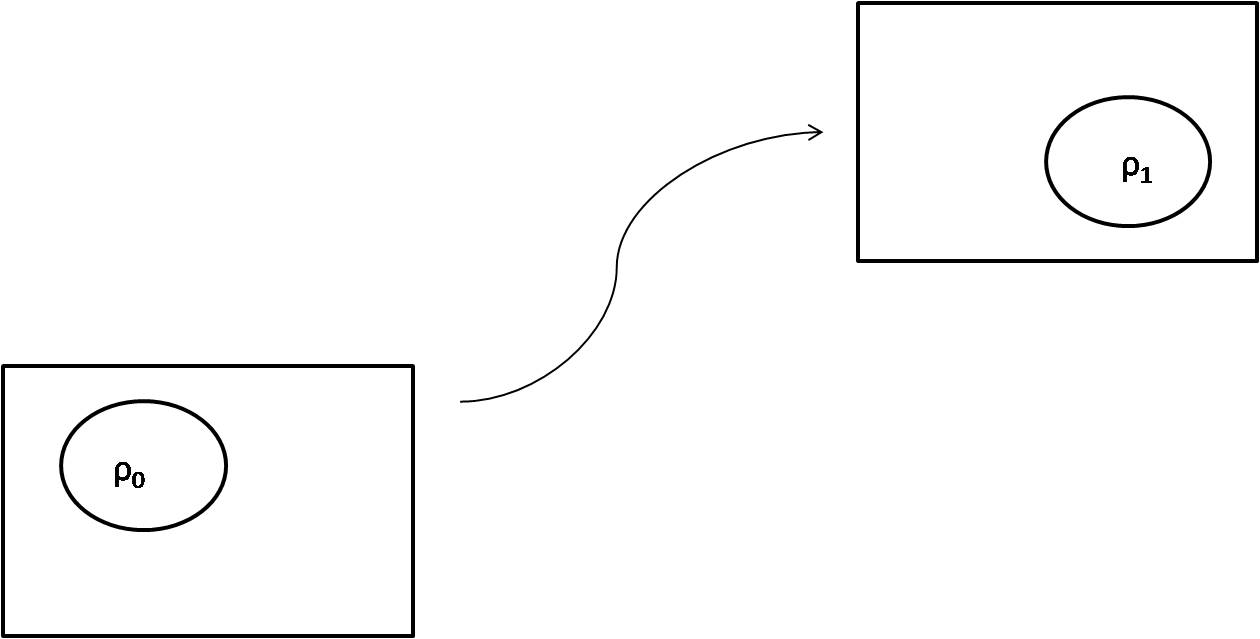
\includegraphics[scale=0.25]{densite.jpg}
    \caption{Transport optimal}
    \end{center}
    \end{figure}


    \end{frame}

    \begin{frame}
    \frametitle{Exemple}
    \begin{figure}
    \begin{center}
    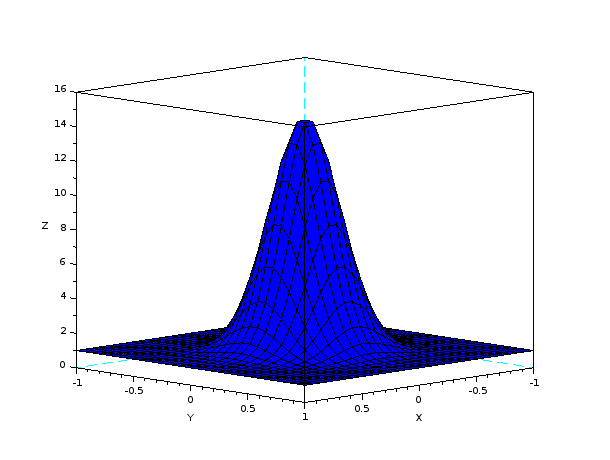
\includegraphics[scale=0.18]{gaussienne.png}
    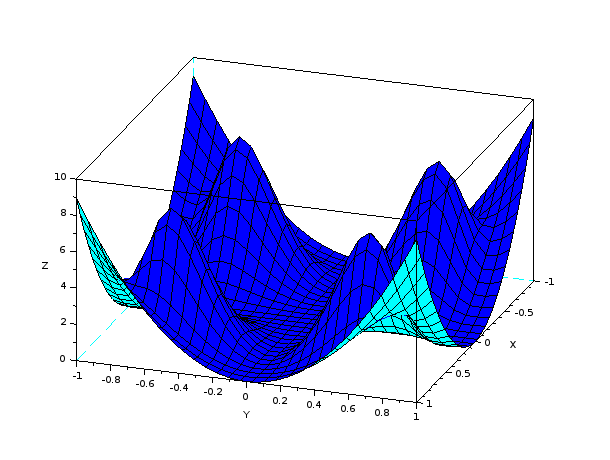
\includegraphics[scale=0.18]{resmapchoisie.png} \\
                           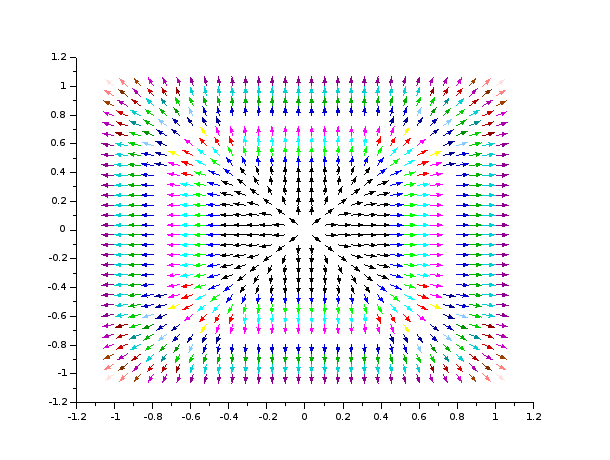
\includegraphics[scale=0.18]{mapchoisie.png} 
                           \caption{Exemple de déplacement de mesure de probabilité}
                           \end{center}
                           \end{figure}

                           \end{frame}


                           \begin{frame}
                           \frametitle{Équation à résoudre}

                           \begin{block}{Équation de Monge-Ampère}
                           $$ \det(D^2 u) = \frac{\rho_X}{\rho_Y(\nabla u)}, \; x \in \Omega $$
                           \end{block}
\bigskip
Objectif : Trouver numériquement une solution de viscosité de 
l'équation de Monge-Ampère
\end{frame}

\begin{frame}
\frametitle{Méthode utilisée}

\begin{itemize}
\item Intérieur du domaine : Itération explicite sur l'équation de Monge-Ampère à l'aide de deux schémas aux différences finies
(un schéma précis et un schéma monotone) \\

    \item Bord du domaine : Équation de Hamilton-Jacobi pour 
    s'assurer que les bords des domaines se transportent de l'un
    sur l'autre
    \end{itemize}

    \end{frame}
    \subsection{Implémentation Scilab}

    \begin{frame}
    \frametitle{Travail réalisé}

    \begin{itemize}
    \item Implémentation du schéma précis \\

    \item Implémentation du schéma au bord \\

    \end{itemize}
    \end{frame}

    \begin{frame}
    \frametitle{Résultats}
    \begin{figure}
    \begin{center}
    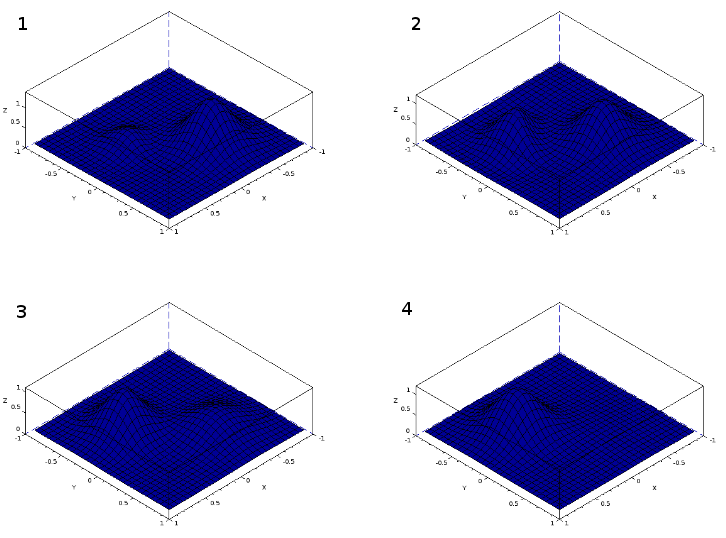
\includegraphics[scale=0.3]{depl1.png}
    \caption{Déplacement d'une Gaussienne}
    \end{center}
    \end{figure}

    \end{frame}

    \begin{frame}
    \frametitle{Résultats}
    \begin{figure}
    \begin{center}
    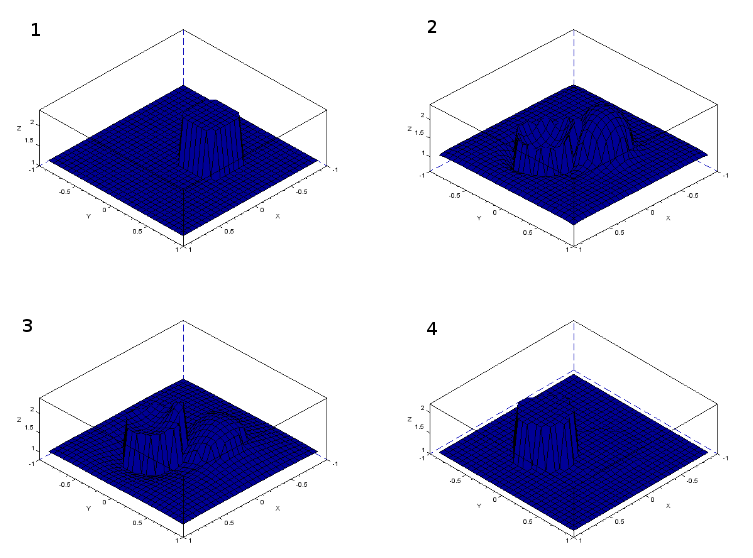
\includegraphics[scale=0.3]{depl2.png}
    \caption{Déplacement d'un disque}
    \end{center}
    \end{figure}
    \end{frame}

    \begin{frame}
    \frametitle{Problème}

    \alert{Le calcul est lent :}
    \begin{itemize}
    \item Utilisation d'une itération explicite

    \item Condition CFL très restreinte

    \item Donc nombre d'itérations nécessaires très élevé
    \end{itemize}
    \end{frame}

    \subsection{Implémentation OpenCL}

    \begin{frame}
    \frametitle{GPU et OpenCL}

    \begin{center}
    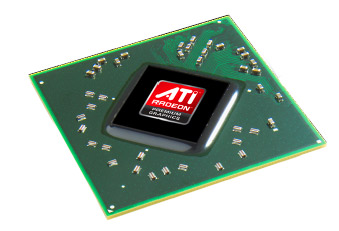
\includegraphics[scale=0.2]{gpu.jpg}
    
\includegraphics[scale=0.2]{opencl.png}
    \end{center}
    \begin{itemize}

    \item Constitué de milliers de petits processeurs\\

    \item Peuvent être programmés avec OpenCL \\

    \item Permet d'exécuter des opérations simples en parallèle \\

    \item<2> \alert{ Parfait pour les différences finies !}

    \end{itemize}
    \end{frame}

    \begin{frame}
    \frametitle{Travail réalisé}

    \begin{itemize}
    \item Implémentation du schéma précis en OpenCL \\

    \item Tests d'exécution sur un GPU intégré de marque Intel et une
    carte graphique AMD
    \end{itemize}

    \end{frame}

    \begin{frame}  
    \frametitle{Résultats}
Gain de performances considérable par rapport à Scilab : \\

\bigskip

    \begin{tikzpicture}
    \node[nodeStyle] (sci) {Scilab\\1m10};
\node[nodeStyle, right = 6cm of sci] (op) {OpenCL\\0.15s};
\draw[->, line width=3pt]  (sci) -- ++(4,0) node[below]{1000 itérations sur 30x30} --  (op);
\end{tikzpicture}

    \begin{tikzpicture}
    \node[nodeStyle] (sci) {Scilab\\8 semaines};
\node[nodeStyle, right = 6cm of sci] (op) {OpenCL\\45s};
\draw[->, line width=3pt]  (sci) -- ++(4,0) node[below]{200000 itérations sur 256x256} --  (op);
\end{tikzpicture}

\bigskip

\alert{L'itération explicite sur GPU est plus rapide que la méthode de 
Newton sur CPU.}
\end{frame}


    \section{Conclusion}

    \begin{frame}
    \frametitle{Bilan}

Travail réalisé :
    \begin{itemize}
    \item Implémentation d'une méthode trouvée dans la littérature \\

    \item Accélération considérable en faisant les calculs sur une carte graphique

    \end{itemize}
\bigskip
Travail restant :
    \begin{itemize}
    \item Débogage du second schéma aux différences finies \\

    \item Portage du second schéma sous OpenCL \\

    \item Implémentation de la méthode de Newton \\


    \end{itemize}
    \end{frame}

    \begin{frame}
    \frametitle{Apport personnel}

    \begin{itemize}
    \item Découverte du monde de la recherche \\

    \item Application d'une démarche scientifique \\


    \end{itemize}

    \end{frame}


    \end{document}
